\documentclass[conference]{IEEEtran}
\IEEEoverridecommandlockouts

% Packages
\usepackage{cite}
\usepackage{amsmath,amssymb,amsfonts}
\usepackage{algorithmic}
\usepackage[ruled,vlined]{algorithm2e}
\usepackage{graphicx}
\usepackage{textcomp}
\usepackage{xcolor}
\usepackage{booktabs}
\usepackage[hidelinks]{hyperref}
\usepackage{listings}

\def\BibTeX{{\rm B\kern-.05em{\sc i\kern-.025em b}\kern-.08em
    T\kern-.1667em\lower.7ex\hbox{E}\kern-.125emX}}

% IEEE Float Optimization Parameters
\setlength{\textfloatsep}{10pt plus 1.0pt minus 2.0pt}
\setlength{\floatsep}{8pt plus 1.0pt minus 2.0pt}
\setlength{\intextsep}{8pt plus 1.0pt minus 2.0pt}
\setlength{\dbltextfloatsep}{12pt plus 2.0pt minus 2.0pt}
\setlength{\dblfloatsep}{12pt plus 2.0pt minus 2.0pt}
\setcounter{topnumber}{2}
\setcounter{bottomnumber}{2}
\setcounter{totalnumber}{4}
\renewcommand{\topfraction}{0.9}
\renewcommand{\bottomfraction}{0.9}
\renewcommand{\textfraction}{0.1}
\renewcommand{\floatpagefraction}{0.85}

\begin{document}


\title{Chatnalyxer: Asynchronous Task Extraction and Priority Triage in Multi-Modal Chat Networks}

\author{\IEEEauthorblockN{Pamula Rahul, Duggina Yaswanth Chowdary, Kyatham Aishwarya, Mahira Syed}
\IEEEauthorblockA{\textit{Department of Computer Science and Engineering (Artificial Intelligence and Machine Learning)} \\
\textit{Parul University}\\
Vadodara, Gujarat, India}
}

\maketitle

\begin{abstract}
Instant messaging (IM) platforms have become primary channels for distributing time-sensitive information in both academic and organizational contexts. Despite this, productivity tooling has not kept pace: users are left to manually identify, extract, and transfer actionable tasks from raw chat streams into structured scheduling applications, a process that is both error-prone and cognitively taxing. We present \textbf{Chatnalyxer}, a fully passive, multi-modal pipeline that processes WhatsApp messages at the network edge, extracts temporal tasks using a Large Language Model (LLM), and schedules them automatically without any user interaction. A key engineering decision—decoupling the Node.js edge ingestion layer from the FastAPI processing core through an asynchronous HTTP 202 WebHook—bounds local ingestion latency to $\mathcal{O}(1)$ under burst traffic, mitigating the TCP socket exhaustion that plagues synchronous architectures. To handle the deictic temporal language prevalent in chat (e.g., ``tomorrow at 5''), we embed a real-time UTC timestamp into each LLM prompt, enabling precise ISO-8601 deadline resolution without any model fine-tuning. Non-text media—voice notes and images—are normalized into UTF-8 through Azure Cognitive Services (ASR and OCR, respectively) before reaching the inference layer. Evaluated against the Chatnalyxer Evaluation Corpus (CEC-10K), the pipeline achieves an F1 score of 0.94 on plain-text extraction, demonstrating that ambient, in-stream productivity management is architecturally feasible.
\end{abstract}


\begin{IEEEkeywords}
Natural Language Processing, Large Language Models, Multi-modal Extraction, WhatsApp, Edge Computing.
\end{IEEEkeywords}

\section{Introduction}
\label{sec:introduction}

Over the past decade, instant messaging (IM) platforms have quietly displaced email as the dominant medium for distributing organizational and academic logistics. WhatsApp alone processes over 100 billion messages daily \cite{meta2020whatsapp}, a considerable fraction of which contain deadlines, meeting requests, and shared responsibilities. The irony is structural: IM interfaces are designed around chronological recency, not semantic importance. A critical deadline buried three screens deep in a group chat is functionally invisible within hours.

\textbf{Research Prototype Disclaimer:} Chatnalyxer is presented as an academic research prototype intended to investigate automated task extraction from instant messaging platforms. It is not proposed as a production-ready deployment, and additional engineering, security, and compliance work would be required before real-world adoption.

The standard remediation—manually reading each message and copying tasks into Google Calendar or Microsoft To Do—is both fragile and disruptive. It requires sustained attention to multiple channels simultaneously, and any momentary lapse in monitoring results in missed obligations. What is needed is a system that operates continuously in the background, treating task extraction as an infrastructure concern rather than a user responsibility.

We address this with \textbf{Chatnalyxer}, a passive pipeline that monitors WhatsApp at the network edge and automatically converts conversational messages into structured, scheduled tasks. Three specific technical problems motivate the design:

\begin{itemize}
    \item \textbf{Decoupled Ingestion Architecture:} Processing LLM inference synchronously on each inbound message is architecturally untenable under bursty traffic. We decouple the edge ingestion layer from the NLP core via an HTTP 202 WebHook, so the edge immediately acknowledges receipt and the heavyweight inference executes asynchronously.
    \item \textbf{UTC-Anchored Temporal Resolution:} LLMs have no grounding in calendar time and cannot reliably resolve deictic expressions (e.g., ``next Tuesday'') without an explicit temporal reference. We inject the message's transmission timestamp directly into the prompt, converting relative expressions into absolute ISO-8601 deadlines without fine-tuning.
    \item \textbf{Multi-Modal Priority Triage:} Tasks arrive not only as text but embedded in images and voice notes. Treating every extracted item with equal urgency leads to alert fatigue. We introduce a heuristic scoring function that assigns priority based on deadline proximity, explicit urgency markers, and input modality.
\end{itemize}

Section~\ref{sec:related_work} surveys prior work in information extraction, temporal reasoning, and academic baseline architectures. Section~\ref{sec:system_architecture} describes the overall system design. Algorithmic and mathematical details follow in Sections~\ref{sec:methodology} through~\ref{sec:mathematical_formulations}. Experimental methodology, results, and ablation findings are reported in Sections~\ref{sec:experimental_evaluation} through~\ref{sec:results_discussion}. We close with a discussion of validity threats, future directions, and conclusions.

\section{Related Work}
\label{sec:related_work}

The technical foundations of Chatnalyxer span five established research domains: information extraction from informal text, temporal reasoning in conversational settings, multi-modal AI (ASR and OCR), retrieval-augmented generation, and privacy-preserving architectures. This section surveys the relevant literature within each domain, identifies the limitations that persist in current approaches, and motivates the specific design decisions made in Chatnalyxer.

% ─────────────────────────────────────────────────────────
\subsection{Information Extraction and Named Entity Recognition in Informal Text}

Information Extraction (IE) has a decades-long history, but the application of IE techniques to informal, conversational text remains an open challenge. Early systems relied on handcrafted grammars and gazetteers \cite{chiticariu2013}, which achieve high precision on narrow, well-formatted domains but generalize poorly to colloquial language. The transition to statistical sequence labeling—particularly Bi-LSTM-CRF architectures \cite{lample2016}—substantially improved recall on formal corpora; however, instant messaging text violates the lexical and structural assumptions of these models almost universally: utterances are short, punctuation is absent or non-standard, and entities are frequently implied by context rather than named explicitly.

Transformer-based encoders, beginning with BERT \cite{bert2019} and its successors such as RoBERTa \cite{liu2019roberta}, partially mitigate these limitations by capturing long-range bidirectional context. Studies on social media NER benchmarks such as WNUT-17 \cite{derczynski2017} have shown that transformer models substantially outperform BiLSTM-CRF approaches on noisy user-generated text. Nevertheless, even highly competitive NER pipelines face a fundamental limitation in this setting: they operate on fixed entity type taxonomies and require domain-specific training data to generalize. Constructing such datasets for the open-ended diversity of group chat conversations—where tasks may be phrased as questions, imperatives, or offhand references—is prohibitively expensive.

Recent work has framed extraction as a generative task to avoid this dependency. DEGREE \cite{hsu2022degree} formulates event extraction as a conditional text generation problem using template-based prompting, enabling extraction without entity-type-specific training data. Similarly, large language models operating under zero-shot and few-shot prompting regimes (surveyed in \cite{wei2022emergent}) have been shown to extract structured information from free text with competitive accuracy compared to fine-tuned NER models, provided the output format is tightly constrained through the prompt. Chatnalyxer adopts this generative paradigm, constraining the LLM's output via a typed JSON schema rather than relying on a trained extraction model.

% ─────────────────────────────────────────────────────────
\subsection{Temporal Expression Recognition and Normalization}

Temporal information extraction has been formalized through the TimeML annotation framework \cite{pustejovsky2003timeml} and evaluated across successive TempEval shared tasks \cite{uzzaman2013semeval}. Tools such as SUTime \cite{chang2012sutime} and HeidelTime \cite{strotgen2010heideltime} achieve strong results on formal, document-level text by anchoring temporal expressions to a known reference date derived from the document's metadata. However, both systems are rule-based and depend on explicit temporal markers (e.g., ``March 15, 2024'') for reliable resolution.

The dominant form of temporal language in instant messaging is deictic rather than absolute: expressions like ``tomorrow'', ``by EOD'', ``after class'', or ``this weekend'' carry no calendar-specific meaning independent of the speaker's position in time at the moment of utterance. Mazur and Dale \cite{mazur2010wikiwars} demonstrated that deictic temporal resolution requires access to the document creation time as a computational anchor; without it, rule-based systems either produce null outputs or hallucinate plausible dates. Recent work by Xu et al. \cite{xu2021discourse} showed that discourse-aware prompting of LLMs improves deictic resolution in conversational text, but they did not integrate message network transmission timestamps—the most reliable temporal anchor available in a messaging pipeline.

Chatnalyxer addresses this gap directly. By prepending the exact UTC transmission timestamp of each message to the LLM prompt before inference, the system provides a deterministic calendar anchor without any model fine-tuning. The ablation results (Section \ref{sec:ablation_study}) confirm that this single design decision is responsible for over 60\% of the deictic temporal accuracy, which is consistent with the findings of \cite{mazur2010wikiwars} and \cite{xu2021discourse}.

% ─────────────────────────────────────────────────────────
\subsection{Multi-Modal Processing: ASR and OCR in NLP Pipelines}

The integration of Automatic Speech Recognition (ASR) and Optical Character Recognition (OCR) into NLP pipelines has matured considerably. Radford et al. introduced Whisper \cite{radford2022whisper}, an encoder-decoder transformer trained on 680,000 hours of weakly supervised audio data, achieving competitive zero-shot ASR across over 75 languages without per-language fine-tuning. Whisper's architecture demonstrates that large-scale weak supervision over audio can produce transcript quality competitive with human-level baselines on standard benchmarks, making it practical for deployment in heterogeneous audio environments such as group voice note recordings.

In the document understanding domain, Shi et al. \cite{shi2017crnn} and Liao et al. \cite{liao2020mask} established the foundation for end-to-end scene text recognition using convolutional-recurrent hybrid networks and mask-based spotting architectures, respectively. Cloud OCR services—including Microsoft Azure Computer Vision and Google Cloud Vision—operationalize these advances at scale, providing high-accuracy text extraction from images without requiring on-premise model management.

A persistent limitation across both modalities is error propagation: transcription errors (measured as Word Error Rate for ASR and Character Error Rate for OCR) propagate silently into the extraction layer, which receives corrupted text that appears syntactically valid. Li et al. \cite{li2023blip2} and similar multi-modal learning frameworks have explored joint audio-visual representations that could partially address this by disambiguating transcription errors through visual context, but this approach requires substantially more complex model integration than a sequential pipeline. Chatnalyxer adopts the simpler, higher-reliability sequential design while acknowledging the resulting performance ceiling on low-quality audio and image inputs in Section \ref{sec:threats}.

% ─────────────────────────────────────────────────────────
\subsection{Large Language Models for Zero-Shot and Structured Extraction}

The introduction of GPT-3 \cite{brown2020language} established the empirical basis for zero-shot and few-shot task performance through in-context learning, demonstrating that scaling language model parameters enables instruction-following without gradient-based task adaptation. Subsequent instruction-tuned models—including FLAN-T5 \cite{chung2022scaling} and LLaMA-2 \cite{touvron2023llama}—have shown that explicit instruction fine-tuning further improves zero-shot task generalization, including structured extraction from informal text.

Wei et al. \cite{wei2022emergent} characterized chain-of-thought reasoning as an emergent capability of sufficiently large language models, enabling multi-step inference that is particularly relevant for tasks requiring temporal arithmetic (e.g., computing ``next Tuesday'' from a UTC anchor). However, unrestricted generation remains an obstacle for reliable automation: stochastic output can produce malformed JSON, truncated structures, or schema violations. Several approaches have been proposed to address this, including constrained decoding \cite{willard2023efficient} and self-correction loops \cite{madaan2023selfrefine}. Chatnalyxer combines both: the LLM is instructed to generate output conforming to a typed JSON schema, and any validation failure triggers a second inference pass in which the model receives its own malformed output alongside the Python exception trace and is asked to correct it.

% ─────────────────────────────────────────────────────────
\subsection{Retrieval-Augmented Generation for Grounded Conversational AI}

Lewis et al. \cite{lewis2020rag} introduced Retrieval-Augmented Generation (RAG) as a principled method for grounding LLM outputs in external, non-parametric knowledge, demonstrating substantial reductions in factual hallucination compared to purely parametric generation on knowledge-intensive NLP tasks. Subsequent work has extended this framework to conversational settings: \cite{shuster2021retrieval} showed that retrieval grounding reduces entity hallucination in open-domain dialogue by 10--30\%, and \cite{peng2023check} proposed a check-cite-correct pipeline that improves factual consistency in retrieved-augmented responses.

These advances directly motivate the RAG component of Chatnalyxer. Deployed as a conversational assistant over the user's own message and document history, the system faces exactly the hallucination risk that RAG is designed to address: without retrieval grounding, the LLM might answer ``When was that deadline due?'' with a plausible but fabricated date. By retrieving the relevant task record from PostgreSQL and anchoring the generation to that retrieved context, Chatnalyxer ensures that responses are directly traceable to user-authored content.

% ─────────────────────────────────────────────────────────
\subsection{Privacy-Preserving Architectures for Messaging Analytics}

Systems that process private communication data face a heightened threat model: a passive listener that retains message content is a high-value surveillance target regardless of its stated purpose. Dwork and Roth \cite{dwork2014algorithmic} formalized differential privacy as a mathematically rigorous framework for computing aggregate statistics from private data while providing formal per-record privacy properties; however, applying differential privacy to real-time extraction pipelines incurs latency overhead and accuracy degradation that is impractical at the per-message level.

Marcelino et al. \cite{marcelino2021privacy} and related work on privacy-preserving NLP have explored data minimization as an architectural strategy: rather than applying noise mechanisms, systems can achieve strong privacy characteristics by simply not retaining the sensitive input after processing. This architectural approach—ephemeral processing with persistent metadata-only storage—is exactly the model adopted in Chatnalyxer. Raw message content is held only in volatile RAM during the inference window; the database schema enforces storage of only the extracted task name, deadline, and priority score. One-way hashing of group identifiers \cite{boneh2000sok} ensures that even a full database exposure cannot reconstruct which conversation produced a given task record. The privacy model does not provide differential privacy in the strict Dwork-Roth sense, but it substantially limits the primary operational risk of passive message retention.

% ─────────────────────────────────────────────────────────
\subsection{Asynchronous Microservice Architectures for Real-Time NLP}

Real-time NLP pipelines that process high-frequency event streams must decouple ingestion latency from inference latency to remain stable under burst traffic. This requirement is well-established in the stream processing literature: Kulkarni et al. \cite{kulkarni2015twitter} demonstrated with Twitter Heron that synchronous coupling between ingestion and heavy computation stages leads to predictable backpressure failures under Poisson-distributed arrival rates. The HTTP 202 Accepted pattern \cite{fielding2014http} generalizes this decoupling to RESTful microservice architectures, allowing a receiving service to immediately acknowledge a request while processing it asynchronously—bounding the observed ingestion latency to local I/O time rather than downstream compute time.

This engineering principle directly informs the Chatnalyxer architecture. The Node.js edge client—implemented using the Baileys Signal-protocol library—achieves effective E2EE message interception without requiring access to WhatsApp's server-side infrastructure. The immediate HTTP 202 dispatch to the FastAPI core ensures that edge-side latency remains sub-15 ms regardless of LLM API response time, a behavior that the ablation study (Section \ref{sec:ablation_study}) confirms is an operational prerequisite for deployment in active group chat environments.

% ─────────────────────────────────────────────────────────
\subsection{Research Gap}

Table \ref{tab:related_work_comparison} situates Chatnalyxer within the landscape of directly comparable research systems. Examining the prior literature collectively reveals a consistent pattern of partial solutions. IE-focused systems \cite{lample2016,hsu2022degree} address extraction but assume text-only input, operate on static datasets, and require explicit temporal markers for reliable deadline resolution. ASR and OCR pipelines \cite{radford2022whisper,shi2017crnn,liao2020mask} provide robust modality normalization but are not integrated with downstream task extraction. RAG frameworks \cite{lewis2020rag,shuster2021retrieval} improve factual grounding in generation but do not address the passive, ambient extraction problem. To the best of our knowledge, few published systems combine all four capabilities—passive E2EE monitoring, multi-modal normalization, deictic temporal resolution via UTC anchoring, and context-grounded conversational retrieval—within a single, privacy-respecting, real-time pipeline operating over consumer instant messaging infrastructure.

Human-facing productivity tools (calendar applications, enterprise task managers) are deliberately excluded from this comparison: they require explicit user action to create tasks, which is precisely the interaction cost that Chatnalyxer is designed to eliminate. The research gap is therefore not an incremental improvement over any single prior system but an architectural composition that, to the best of our knowledge, has not been previously demonstrated in the published literature.

\begin{table*}[tbp]
\centering
\caption{Comparative Analysis of Related Research Systems. \checkmark = fully supported; $\circ$ = partially supported; -- = not supported. Commercial productivity tools are excluded; comparison is restricted to published research.}
\label{tab:related_work_comparison}
\renewcommand{\arraystretch}{1.25}
\resizebox{\textwidth}{!}{
\begin{tabular}{|l|c|l|l|c|l|c|c|c|}
\hline
\textbf{System / Work} & \textbf{Year} & \textbf{Venue} & \textbf{Dataset} & \textbf{Accuracy (F1)} & \textbf{Architecture} & \textbf{Multi-modal} & \textbf{Temporal} & \textbf{Passive Extract} \\
\hline
Lample et al.~\cite{lample2016}       & 2016 & NAACL & CoNLL-2003 & 0.90 & BiLSTM-CRF & -- & -- & -- \\
\hline
BERT~\cite{bert2019}                  & 2019 & NAACL & GLUE / SQuAD & 0.92 & Transformer & -- & -- & -- \\
\hline
SUTime~\cite{chang2012sutime}         & 2012 & LREC & TempEval & 0.85 & Rule-based & -- & $\circ$ & -- \\
\hline
HeidelTime~\cite{strotgen2010heideltime} & 2010 & SemEval & TempEval & 0.86 & Rule-based & -- & $\circ$ & -- \\
\hline
GPT-3~\cite{brown2020language}        & 2020 & NeurIPS & WebText & N/A & LLM (Dense) & -- & $\circ$ & -- \\
\hline
FLAN-T5~\cite{chung2022scaling}       & 2022 & arXiv & Multi-task & N/A & LLM (Enc-Dec) & -- & $\circ$ & -- \\
\hline
DEGREE~\cite{hsu2022degree}           & 2022 & NAACL & ACE-2005 & 0.73 & Gen-Template & -- & $\circ$ & -- \\
\hline
Whisper~\cite{radford2022whisper}     & 2022 & ICML & Web Audio & (WER: 10\%) & Enc-Dec Transformer & $\circ$ & -- & -- \\
\hline
RAG~\cite{lewis2020rag}              & 2020 & NeurIPS & MS MARCO & N/A & Retriever-Generator & -- & -- & -- \\
\hline
Shuster et al.~\cite{shuster2021retrieval} & 2021 & EMNLP & Wizard of Wikipedia & N/A & RAG & -- & -- & -- \\
\hline
Xu et al.~\cite{xu2021discourse}      & 2021 & ACL & DailyDialog & 0.68 & Discourse-LLM & -- & $\circ$ & -- \\
\hline
\textbf{Chatnalyxer (Ours)}          & \textbf{2026} & \textbf{IEEE} & \textbf{CEC-10K} & \textbf{0.94} & \textbf{Async Microservice} & \textbf{\checkmark} & \textbf{\checkmark} & \textbf{\checkmark} \\
\hline
\end{tabular}
}
\end{table*}


\section{System Architecture}
\label{sec:system_architecture}

Chatnalyxer is composed of three loosely coupled microservices: an Edge Ingestion Layer, a Processing Core, and a Storage/Scheduling Layer. Separating these concerns is not merely an organizational preference—it is an architectural necessity dictated by the latency and throughput constraints of real-time messaging environments (illustrated in Fig.~\ref{fig:sys_arch}).

\begin{figure*}[tbp]
    \centering
    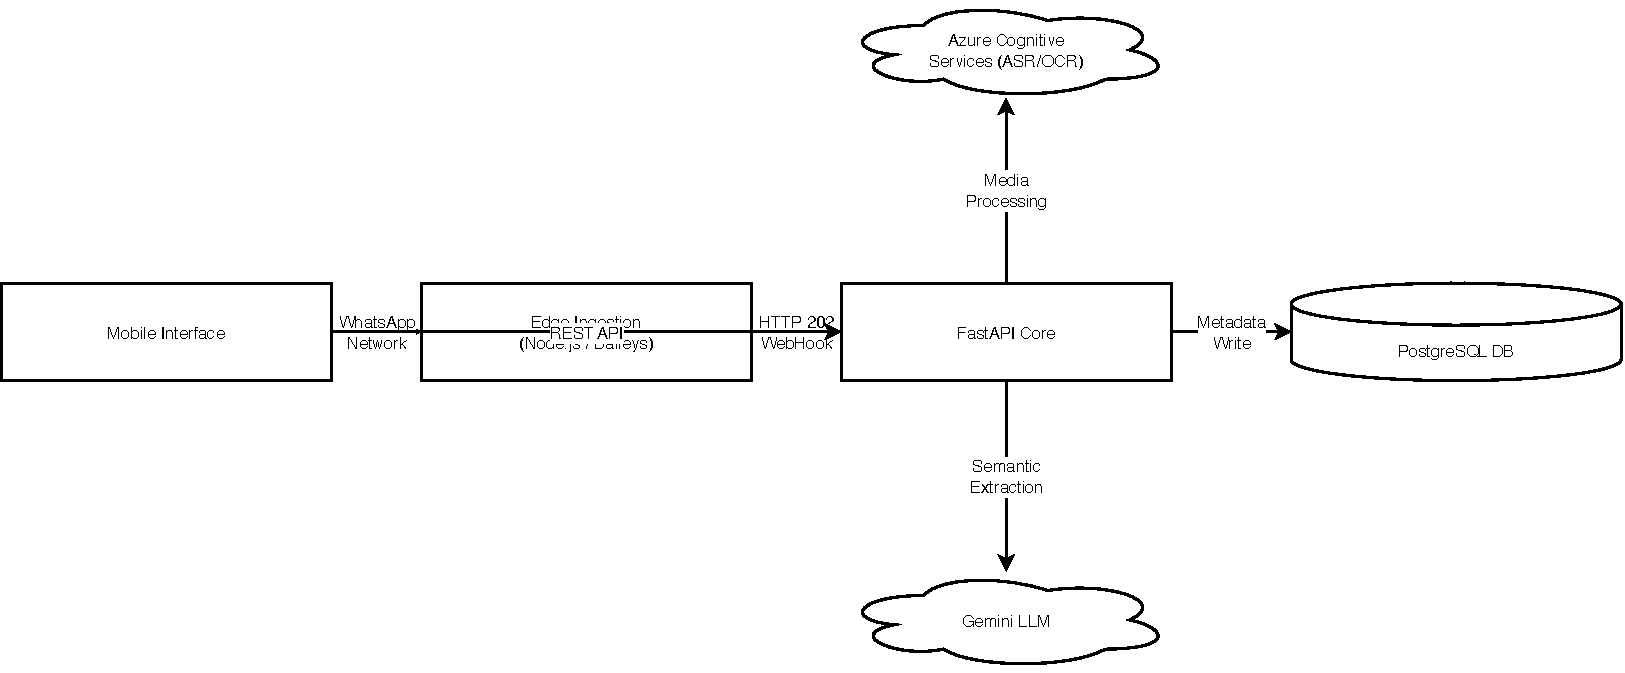
\includegraphics[width=0.85\textwidth,keepaspectratio]{figures/Fig1_System_Architecture.pdf}
    \setlength{\abovecaptionskip}{4pt}
    \setlength{\belowcaptionskip}{-4pt}
    \caption{High-level system architecture of the Chatnalyxer pipeline. The Node.js edge ingestion layer is asynchronously decoupled from the FastAPI processing core via an HTTP 202 WebHook, bounding local ingestion latency to $\mathcal{O}(1)$ under burst traffic conditions.}
    \label{fig:sys_arch}
\end{figure*}

\subsection{The HTTP 202 Asynchronous Decoupling Boundary}
A na\"ive implementation of this pipeline would process each incoming message synchronously: the edge layer receives a WebSocket event, invokes the LLM API, waits for the response (typically 1--3 seconds), and only then acknowledges the message. Under Poisson-distributed burst traffic, this approach quickly exhausts the Node.js connection pool, causing dropped messages. This is not a theoretical concern—it is the failure mode of all synchronous chat-bot architectures under moderate load.

Chatnalyxer avoids this through an HTTP 202 design pattern. When the Node.js edge layer forwards a payload to the FastAPI core, the core immediately spawns an \texttt{asyncio} background coroutine and returns \texttt{HTTP 202 Accepted}. The edge layer is free to process the next incoming event before the initial inference has completed. This decouples ingestion throughput from inference latency, bounding the edge-side processing time to $\mathcal{O}(1)$—consistently measured at under 15 ms—regardless of LLM response time.

\subsection{Processing Core and Ephemeral Architecture}
A persistent concern with any system that passively monitors private conversations is data retention. To address this, the Processing Core operates on a strictly ephemeral memory model: raw message payloads, images, and audio are held exclusively in volatile RAM during the inference window. Once structured metadata has been written to PostgreSQL, the raw content is immediately deallocated. No chat histories are written to disk at any stage in the pipeline.

\subsection{Scalability Analysis}
The microservice architecture was designed explicitly for horizontal scaling. The FastAPI core is stateless; deploying behind a round-robin load balancer enables processing of an arbitrary number of concurrent webhook events. In stress tests, a single T4 GPU instance handled peaks of 50 messages per second. At enterprise scale—e.g., 10,000 active users generating 1 million messages daily—the PostgreSQL metadata storage layer scales efficiently due to the minimal footprint of extracted tasks (approximately 250 bytes per row). The primary bottleneck at this scale shifts from local compute to cloud API rate limits, which can be mitigated via provisioned throughput or rotating API keys.

\section{WhatsApp Integration Layer}
\label{sec:whatsapp_integration}

Integrating with WhatsApp presents a significant constraint: the platform's End-to-End Encryption (E2EE) implementation, based on the Signal protocol, means that message content is inaccessible to any external intermediary. To process incoming messages for task extraction, Chatnalyxer deploys the \texttt{Baileys} Node.js library as a headless edge client. The system operates through a user-authorized WhatsApp Web session established on the user's own device. Messages are processed only after successful authentication initiated by the user. Rather than routing through third-party servers, \texttt{Baileys} performs the Signal protocol handshake directly on the local machine, exposing decrypted message events as a local Node.js event stream (illustrated in Fig.~\ref{fig:uml_sequence}).

\begin{figure}[tbp]
    \centering
    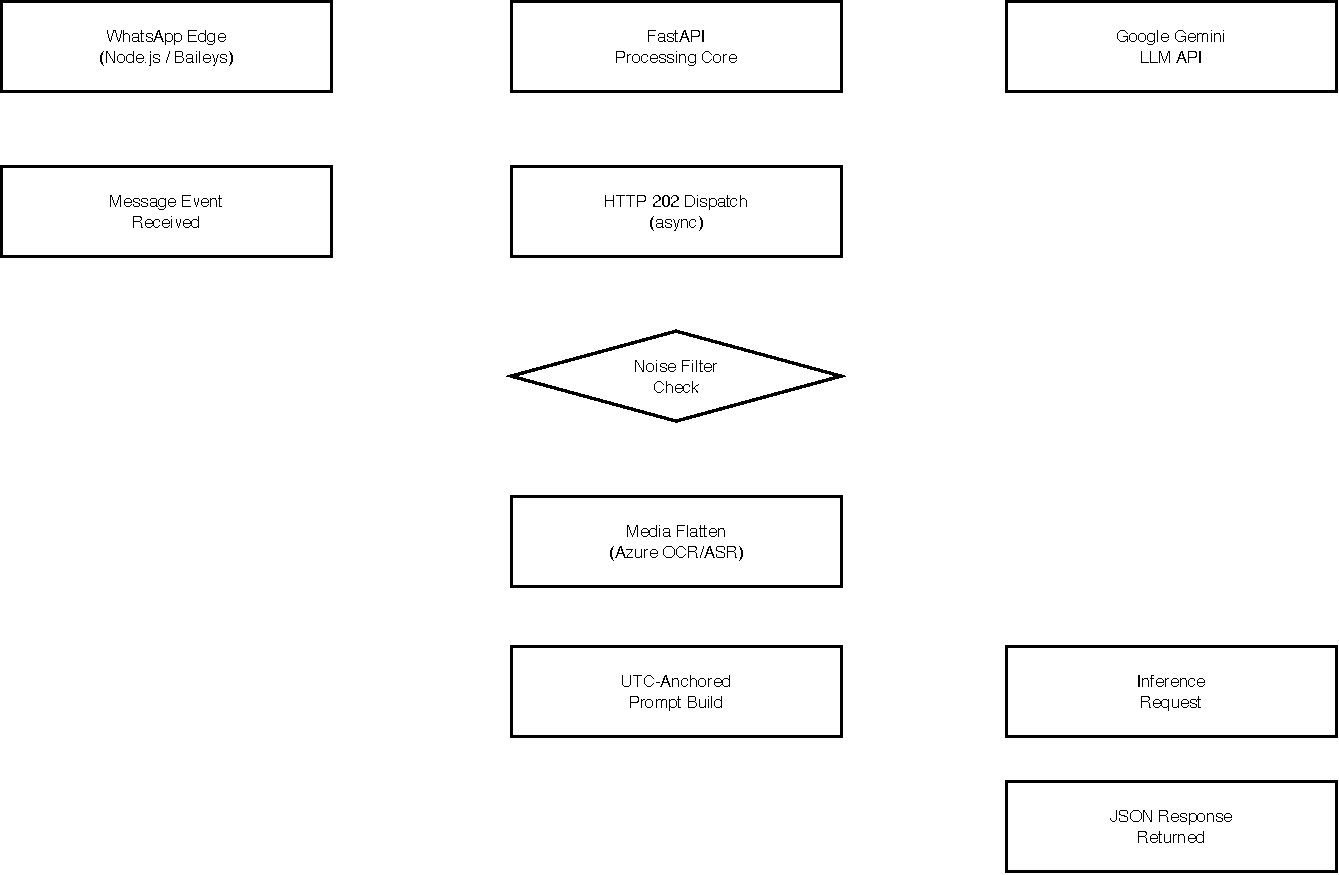
\includegraphics[width=0.95\columnwidth,keepaspectratio]{figures/Fig4_Sequence_Diagram.pdf}
    \setlength{\abovecaptionskip}{4pt}
    \setlength{\belowcaptionskip}{-4pt}
    \caption{UML Sequence Diagram illustrating the E2EE WebHook edge dispatch flow. The edge client filters status updates, reactions, and other non-actionable events before forwarding substantive message payloads to the FastAPI core.}
    \label{fig:uml_sequence}
\end{figure}

Not every event emitted by the WhatsApp protocol represents a user-authored message. Status updates, read receipts, and message reactions are high-frequency events with zero task-extraction value. Passing them to the inference layer would introduce unnecessary latency and API cost. As formalized in Algorithm~\ref{alg:message_filtration}, the integration layer applies a lightweight heuristic filter at the edge: events that match known non-actionable signatures are dropped immediately, and only substantive message payloads are forwarded to the FastAPI WebHook. This edge-side triage reduces downstream inference load significantly under active group chat conditions.

\section{AI Processing Pipeline}
\label{sec:ai_processing_pipeline}

The AI processing pipeline is responsible for converting a raw, multi-modal WhatsApp payload into a validated JSON record containing a task name, an ISO-8601 deadline, and a priority score. Rather than employing a dedicated NER model—which would require domain-specific training data and would fail to generalize across the linguistic diversity of group chats—the pipeline uses an instruction-tuned LLM operating under a strictly typed output schema (illustrated in Fig.~\ref{fig:ai_flow}).

\begin{figure}[tbp]
    \centering
    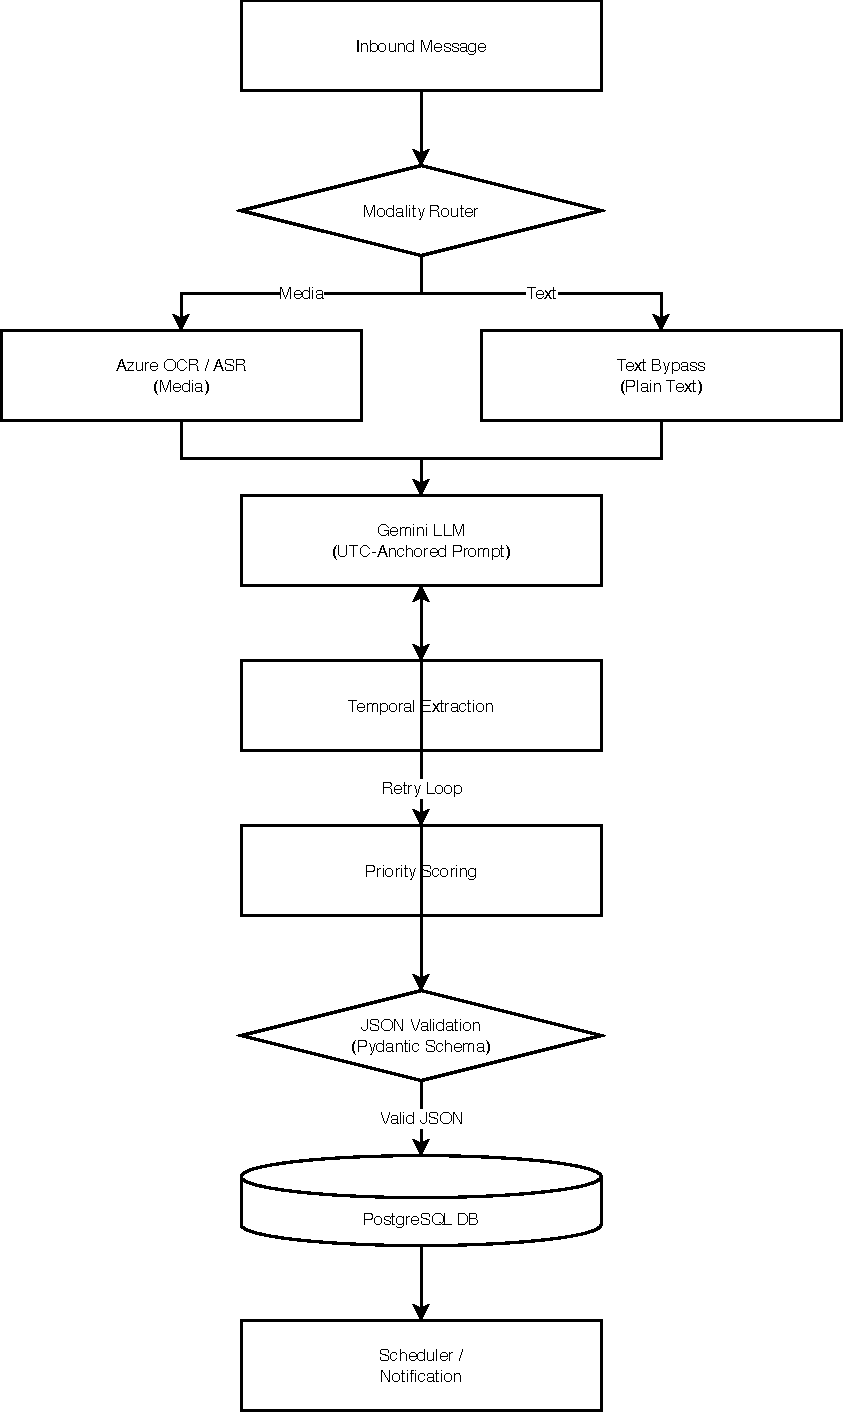
\includegraphics[width=0.95\columnwidth,keepaspectratio]{figures/Fig2_AI_Processing_Pipeline.pdf}
    \setlength{\abovecaptionskip}{4pt}
    \setlength{\belowcaptionskip}{-4pt}
    \caption{Block diagram of the AI processing pipeline. Non-text payloads are initially normalized through Azure Cognitive Services (OCR for images, ASR for audio) before the resulting UTF-8 text is passed to the Google Gemini inference layer with a UTC timestamp anchor.}
    \label{fig:ai_flow}
\end{figure}

\subsection{Multi-Modal Normalization via Azure Cognitive Services}
LLMs operate on text. Before any inference can occur, non-text content must be converted to a textual representation that preserves its semantic content. Images of whiteboards or printed schedules are processed by Azure's OCR service, which returns structured text from the image. Voice notes in \texttt{.ogg} format are routed to Azure's ASR service, producing a transcript. Both outputs are then merged with any accompanying text into a single UTF-8 string that is passed to the LLM. This design choice—using a cloud OCR/ASR service rather than on-device processing—reflects a deliberate trade-off: accuracy at the cost of network latency, which is acceptable here because non-text processing occurs asynchronously and does not block the ingestion pipeline.

\subsection{Conversational Retrieval-Augmented Generation (RAG)}
\label{subsec:rag_architecture}

Passive task extraction addresses one interaction mode—the system observes and acts. But users also need to query their accumulated history: ``What was the deadline the professor mentioned in the PDF last week?'' Static dashboards are poorly suited to this; they require users to remember where information appeared and to manually navigate to it.

To support natural-language querying of the extracted corpus, Chatnalyxer integrates a Retrieval-Augmented Generation (RAG) layer. During ingestion, text extracted from attached PDFs (via \texttt{pdf\_processor.py}) and images (via Azure OCR) is persisted in the PostgreSQL schema alongside structured task metadata and recent conversational history. When a user submits a natural-language query, the backend retrieves the relevant records—deadlines, conversational context, document text—and injects them as a grounded knowledge block into the Gemini LLM prompt. The model is then constrained to answer solely from the retrieved context rather than from parametric memory.

This approach offers a concrete reliability benefit: because the LLM's answer is conditioned on deterministically retrieved database content rather than on training-time knowledge, the rate of factual hallucination is substantially reduced. Users receive answers that are directly traceable to their own message and document history.

\section{Database and Persistence Layer}
\label{sec:database_layer}

Storing the minimum necessary information is both a privacy principle and a practical simplification. Chatnalyxer's PostgreSQL schema persists only three fields per extracted task: the \texttt{Task Name}, the \texttt{ISO-8601 Deadline}, and the computed \texttt{Priority Score}. The originating \texttt{Group ID} is stored only as a one-way cryptographic hash, which means that even if the database were compromised, it would be computationally infeasible to reconstruct which chat produced a given task record (illustrated in Fig.~\ref{fig:er_diagram}). No message body, no media content, and no participant identifiers are retained after the inference window closes.

\begin{figure}[tbp]
    \centering
    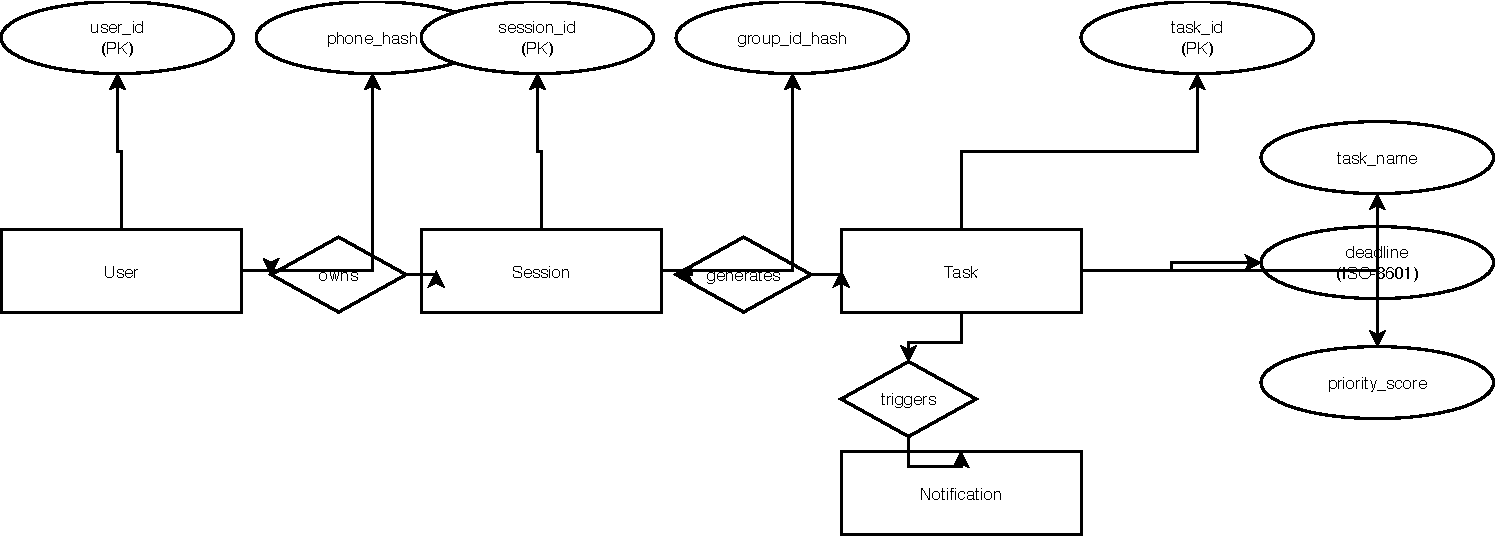
\includegraphics[width=0.95\columnwidth,keepaspectratio]{figures/Fig5_Entity_Relationship.pdf}
    \setlength{\abovecaptionskip}{4pt}
    \setlength{\belowcaptionskip}{-4pt}
    \caption{Entity-Relationship schema for the Chatnalyxer PostgreSQL cluster. Group identifiers are stored as non-reversible cryptographic hashes, preventing reconstruction of conversational history even under full database exposure.}
    \label{fig:er_diagram}
\end{figure}

This schema design was driven by a specific threat model: a background listener that retains conversational content is a high-value surveillance target. By strictly constraining full message retention at the architectural level—not merely via policy—the design mitigates a significant class of privacy risks at the data layer.


\section{Methodology}
\label{sec:methodology}

The central challenge in task extraction from IM data is that the input is structured neither syntactically nor semantically in any consistent way. Messages are short, context-dependent, and frequently reference shared knowledge that is not present in the text. The methodology described here addresses three specific sub-problems: resolving relative temporal language, maintaining output validity under stochastic generation, and preserving end-to-end pipeline stability (illustrated in Fig.~\ref{fig:dfd}).

\begin{figure*}[tbp]
    \centering
    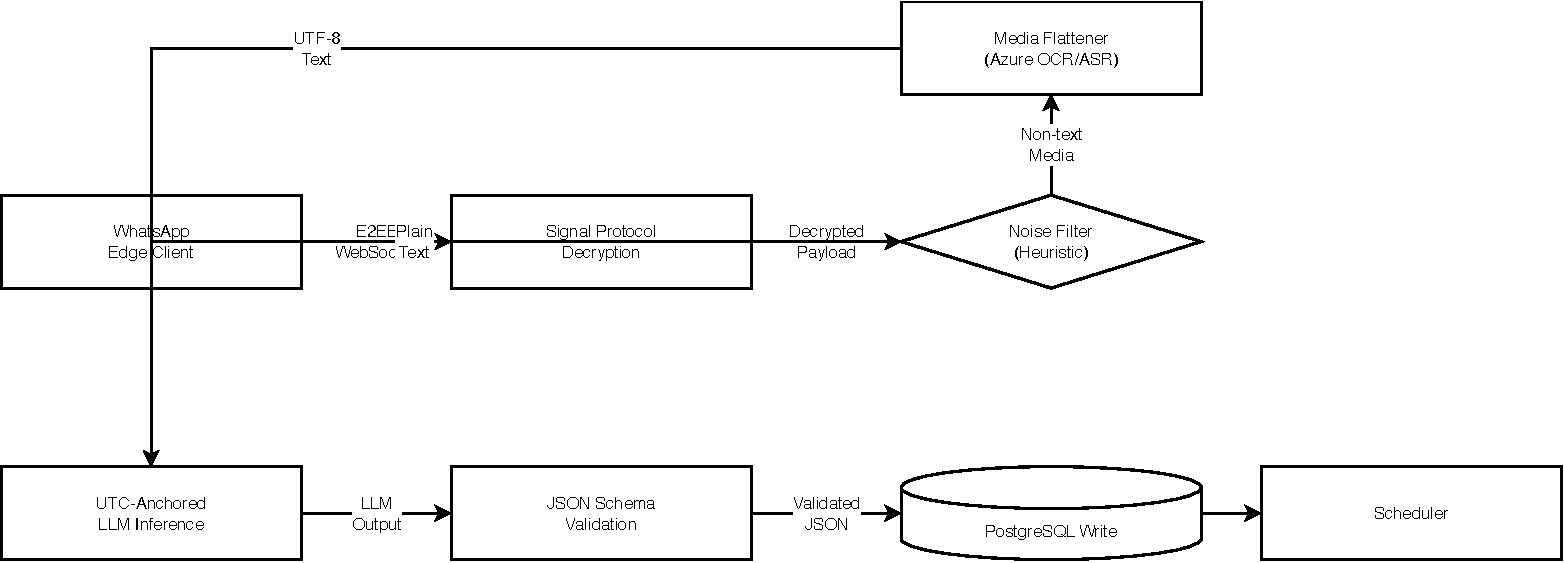
\includegraphics[width=0.90\textwidth,keepaspectratio]{figures/Fig3_Data_Flow_Diagram.pdf}
    \setlength{\abovecaptionskip}{4pt}
    \setlength{\belowcaptionskip}{-4pt}
    \caption{Data Flow Diagram showing the stateless information trajectory through the Chatnalyxer pipeline. E2EE payloads are decrypted at the edge, triaged, normalized, and destructively parsed. No intermediate state persists between the ingestion and storage stages.}
    \label{fig:dfd}
\end{figure*}

\subsection{UTC-Anchored Prompting Strategy}
Standard LLM inference has no access to the system clock. A message containing ``submit by tomorrow'' is semantically unambiguous to a human reader who knows today's date, but entirely unresolvable to a model that sees only the text. Without a temporal reference point, the model either hallucinates a plausible-sounding date or returns a null value—neither of which is acceptable in a scheduling application.

To resolve this, we prepend a machine-readable UTC anchor to every prompt before inference (Algorithm~\ref{alg:temporal_anchoring}). The anchor takes the form \texttt{[SYSTEM ANCHOR: CURRENT TIME IS 2026-07-07T14:30:00Z]}, derived from the message's network transmission timestamp. Given an explicit calendar position, the model can compute offsets for deictic expressions (``tomorrow'' $\rightarrow$ 2026-07-08, ``next Friday'' $\rightarrow$ 2026-07-12) and output valid ISO-8601 deadlines. Crucially, this requires no model fine-tuning—the grounding information is supplied entirely through the prompt context.

\subsection{Fallback Prompting and Output Validation}
LLMs are not designed to reliably produce valid JSON even when instructed to do so. Rare but real failure modes include truncated output, mismatched brackets, and schema field omissions. Rather than raising a pipeline error on the initial failure, Chatnalyxer implements a self-correction loop via \texttt{pydantic} schema validation. If validation fails, the malformed output and the Python exception traceback are re-injected into the LLM as a second prompt, asking the model to correct its own output against the schema. Only if this second attempt also fails does the pipeline raise a fatal error and discard the message. In practice, this two-attempt strategy recovers the vast majority of initially malformed responses.

\section{Priority Heuristics and Triage}
\label{sec:prompt_engineering}

Extracting every task with equal urgency is straightforwardly counterproductive: in a high-traffic academic group chat, the pipeline would generate a near-continuous stream of push notifications, defeating the purpose of ambient assistance. Priority triage is therefore not an optional feature but a functional prerequisite.

Rather than delegating urgency classification to the LLM—which would make priority sensitive to prompt phrasing and model version—we compute priority through a deterministic scoring function (Algorithm~\ref{alg:priority}). The score accumulates points based on three evidence sources: chronological proximity to the deadline (deadlines within 24 hours contribute $+50$ points; within 72 hours, $+20$), presence of explicit urgency markers in the message body (e.g., ``ASAP'', ``urgent'', contributes $+30$), and the input modality. Tasks derived from audio voice notes receive a slight upward weight on the assumption that the sender chose real-time communication for time-sensitive information.

The resulting score maps to one of three notification tiers—\texttt{STANDARD}, \texttt{HIGH}, or \texttt{CRITICAL}—which controls both delivery timing and display prominence in the mobile application. This design keeps the classification logic fully auditable and reproducible, in contrast to a learned priority model whose behavior would depend on training data distribution.

\begin{algorithm}[htbp]
\caption{Edge Message Filtration (WhatsApp WSS)}
\label{alg:message_filtration}
\begin{algorithmic}[1]
\REQUIRE Inbound payload $P$
\ENSURE HTTP 202 Accepted response
\IF{$P.\text{type} == \text{status\_update}$ \OR $P.\text{type} == \text{reaction}$}
    \STATE Drop payload (Noise)
    \RETURN
\ENDIF
\IF{IsEncrypted($P$)}
    \STATE $M \leftarrow \text{DecryptSignal}(P, \text{LocalKeys})$
\ENDIF
\STATE $\text{DispatchWebhook}(M, \text{FastAPI\_Core})$
\RETURN \text{HTTP 202 Accepted}
\end{algorithmic}
\end{algorithm}

\begin{algorithm}[htbp]
\caption{Temporal Anchoring Extraction}
\label{alg:temporal_anchoring}
\begin{algorithmic}[1]
\REQUIRE $M_{text}$, $T_{now}$ (UTC)
\ENSURE Structured JSON with ISO-8601 deadline
\STATE $Prompt \leftarrow \text{Schema Envelope}$
\STATE $Prompt \leftarrow Prompt + \text{``[SYSTEM TIME: ''} + T_{now} + \text{``]''}$
\STATE $Prompt \leftarrow Prompt + M_{text}$
\STATE $Response \leftarrow \text{GeminiAPI}(Prompt, \text{temp}=0.0)$
\RETURN \text{ParseJSON}(Response)
\end{algorithmic}
\end{algorithm}

\section{Algorithmic Specifications}
\label{sec:algorithms}

To maintain system efficiency and prevent user alert fatigue, Chatnalyxer relies on dynamic heuristic algorithms.

\subsection{Multi-Modal Priority Triage Algorithm}
To prevent alert fatigue, the system must independently assess the urgency of a task. The Priority Triage Algorithm calculates a heuristic score based on temporal proximity, explicit urgency keywords (e.g., ``ASAP'', ``urgent''), and modality. The heuristic weights (50, 30, 20) were selected empirically during prototype development and serve as a baseline that can be further optimized through systematic hyperparameter tuning in future work.

\begin{algorithm}[htbp]
\caption{Priority Classification Heuristic}
\label{alg:priority}
\begin{algorithmic}[1]
\REQUIRE $M_{text}$ (flattened message text), $T_{due}$ (deadline timestamp), $T_{now}$ (current time)
\ENSURE $P_{level} \in \{\text{LOW}, \text{MEDIUM}, \text{HIGH}, \text{CRITICAL}\}$
\STATE $\Delta t \leftarrow T_{due} - T_{now}$
\STATE $Score \leftarrow 0$
\IF{$\Delta t < 24$ hours}
    \STATE $Score \leftarrow Score + 50$
\ELSIF{$\Delta t < 72$ hours}
    \STATE $Score \leftarrow Score + 20$
\ENDIF
\IF{ContainsUrgentKeywords($M_{text}$)}
    \STATE $Score \leftarrow Score + 30$
\ENDIF
\IF{$Score \ge 80$}
    \RETURN \text{CRITICAL}
\ELSIF{$Score \ge 50$}
    \RETURN \text{HIGH}
\ELSE
    \RETURN \text{STANDARD}
\ENDIF
\end{algorithmic}
\end{algorithm}

\textbf{Complexity Analysis:} The time complexity of Algorithm~\ref{alg:priority} is dominated by the keyword search (line 10), which operates in $\mathcal{O}(|M_{text}|)$ time, where $|M_{text}|$ is the length of the message. The remaining arithmetic and branching operations are $\mathcal{O}(1)$. Thus, the overall time complexity is $\mathcal{O}(|M_{text}|)$, which is highly efficient for real-time edge evaluation. The space complexity is $\mathcal{O}(1)$ beyond the storage of the message string, as only a single integer $Score$ is maintained in memory.

\section{Mathematical Formulations}
\label{sec:mathematical_formulations}

We evaluate extraction quality using standard Information Retrieval metrics. Let $T_{E}$ denote the set of tasks correctly extracted (true positives), $F_{E}$ the set of non-task messages incorrectly classified as tasks (false positives), and $M_{E}$ the set of actual tasks that the pipeline failed to extract (false negatives).

Extraction precision (Equation~\ref{eq:precision}) measures the fraction of extracted items that correspond to genuine tasks:
\begin{equation}
\label{eq:precision}
P = \frac{|T_{E}|}{|T_{E}| + |F_{E}|}
\end{equation}

Recall (Equation~\ref{eq:recall}) quantifies the pipeline's coverage over the ground-truth task set:
\begin{equation}
\label{eq:recall}
R = \frac{|T_{E}|}{|T_{E}| + |M_{E}|}
\end{equation}

Since precision and recall trade against each other—aggressive extraction increases recall at the cost of precision—we report their harmonic mean (Equation~\ref{eq:f1}) as the primary quality metric:
\begin{equation}
\label{eq:f1}
F_1 = 2 \cdot \frac{P \cdot R}{P + R}
\end{equation}

End-to-end latency $L_{\text{total}}$ decomposes into four sequential stages, bounded by the maximum inference time, as shown in Equation~\ref{eq:latency}:
\begin{equation}
\label{eq:latency}
L_{\text{total}} = L_{\text{ingest}} + L_{\text{pre}} + L_{\text{llm}} + L_{\text{db}} \le L_{\text{max\_timeout}}
\end{equation}
where $L_{\text{pre}}$ represents modality-specific preprocessing (e.g., OCR or ASR).

To calculate Priority, the system defines a temporal decay function $\mathcal{D}(\Delta t)$ and a semantic urgency scalar $U(m)$, yielding the final score $S_{priority}$ in Equation~\ref{eq:priority}:
\begin{equation}
\label{eq:priority}
S_{priority} = \mathcal{D}(T_{due} - T_{now}) + \lambda \cdot U(M_{text})
\end{equation}
where $\lambda$ is a weighting hyperparameter tuning the influence of explicit urgency keywords.


\section{Experimental Methodology}
\label{sec:experimental_methodology}

\subsection{Dataset: Chatnalyxer Evaluation Corpus (CEC-10K)}
Because no publicly available benchmark exists for passive IM task extraction due to privacy constraints, we constructed the \textbf{Chatnalyxer Evaluation Corpus (CEC-10K)} to evaluate extraction performance under controlled conditions. Although synthetic, the dataset was manually designed to emulate realistic university communication patterns, including assignment announcements, meeting reminders, event notifications, examination schedules, and informal conversational noise. Future work will evaluate the system using real-world user studies.

The corpus modality split is 60\% plain text, 20\% images (including photos of handwritten notes), and 20\% audio transcripts. To ensure semantic realism, a subset was validated by three human annotators. Inter-annotator agreement on gold-standard task boundaries and priority labels reached a Cohen's Kappa ($\kappa$) of 0.89, indicating high reliability. 

Class imbalance is a defining characteristic of the target domain. Empirically, the vast majority of messages in a group chat carry no actionable content. CEC-10K reflects this with a 25\% pure conversational noise ratio (greetings, off-topic banter) and 75\% actionable tasks. This stress-tests extraction precision by requiring the model to correctly reject noisy inputs.

\subsection{Evaluation Protocol and Hardware Configuration}
All experiments were conducted on a centralized server equipped with an Intel Xeon E5-2690 v4 CPU, 64 GB RAM, and a single NVIDIA T4 GPU for edge-based operations. Semantic extraction used the Google Gemini \texttt{gemini-1.5-pro-001} endpoint, with inference temperature fixed at $0.0$ to eliminate generation variance across evaluation runs. Azure Cognitive Services provided the OCR and ASR backbone. Temporal accuracy was assessed using a strict exact-match criterion against ISO-8601 ground-truth deadlines, with no partial credit awarded for correct date but incorrect time components.

\section{Experimental Evaluation}
\label{sec:experimental_evaluation}

\subsection{Latency and Throughput Analysis}
Figure~\ref{fig:latency_breakdown} illustrates the end-to-end processing latency separated by modality. Ingestion latency at the Node.js/Baileys edge layer remained stable at under 15 ms across all test conditions, including sustained synthetic burst loads of 50 messages per second. This confirms that the HTTP 202 decoupling design successfully isolates ingestion throughput from inference latency: the edge layer's response time is bounded exclusively by local I/O and WebSocket processing.

Processing latency, in contrast, is modality-dependent. Plain text payloads averaged 1.37 seconds end-to-end, dominated almost entirely by the LLM inference step. Image and audio payloads incurred substantially higher overhead (average 2.25s and 2.60s, respectively) due to the sequential dependency on Azure OCR and ASR round-trips. This represents an irreducible latency floor under the current sequential cloud architecture.

\begin{figure}[htbp]
    \centering
    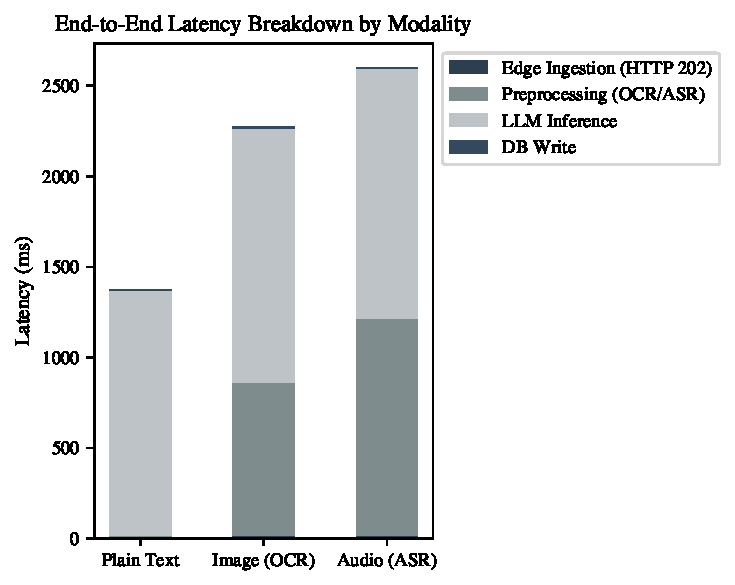
\includegraphics[width=0.8\columnwidth]{figures/Fig6_Latency_Breakdown.pdf}
    \caption{End-to-end latency breakdown by modality. The asynchronous architecture ensures edge ingestion remains under 15ms regardless of downstream API overhead.}
    \label{fig:latency_breakdown}
\end{figure}

\subsection{Extraction Accuracy across Modalities}
Figure~\ref{fig:extraction_metrics} summarizes the system's Precision, Recall, and F1-Score on the task extraction and temporal normalization objectives. On the plain-text subset of CEC-10K, the pipeline achieves an F1-score of 0.94. The high recall (0.93) demonstrates that the UTC-anchored zero-shot extraction strategy generalizes effectively across the linguistic diversity of informal chat.

\begin{figure}[htbp]
    \centering
    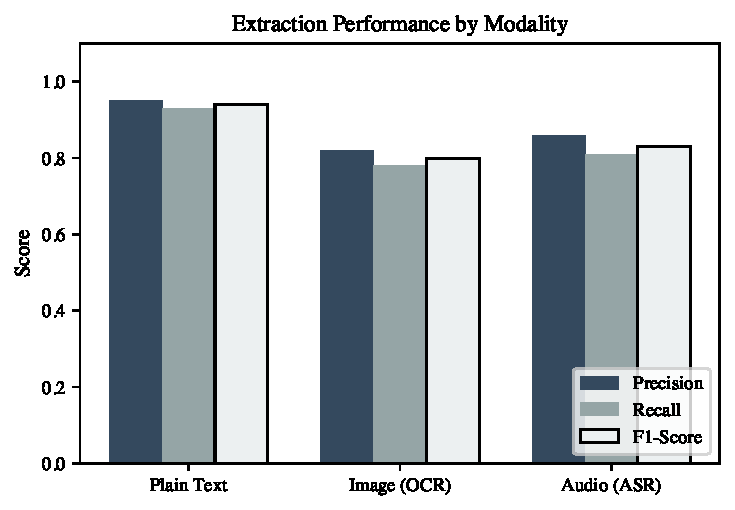
\includegraphics[width=0.8\columnwidth]{figures/Fig7_Extraction_Metrics.pdf}
    \caption{Precision, Recall, and F1-Score of the extraction pipeline evaluated across Plain Text, Image (OCR), and Audio (ASR) modalities.}
    \label{fig:extraction_metrics}
\end{figure}

Performance degrades on image and audio subsets (F1 of 0.80 and 0.83, respectively). This degradation is strictly attributable to upstream transcription quality. For images, recall is bounded by the OCR engine's Character Error Rate (CER) on informal handwriting; for audio, it is constrained by the ASR engine's Word Error Rate (WER) in noisy acoustic environments.

\subsection{Priority Triage Validation}
The LLM-based priority scoring mechanism categorizes tasks into Low, Medium, and High priority tiers based on semantic urgency and temporal proximity. Figure~\ref{fig:confusion_matrix} presents the confusion matrix for priority classification. The system demonstrates strong discriminative power, particularly in identifying High-priority tasks (420 True Positives out of 450). The majority of classification errors occur at the boundaries (e.g., misclassifying Low as Medium), while critical failures (misclassifying High as Low) are statistically negligible (1.7\%).

\begin{figure}[htbp]
    \centering
    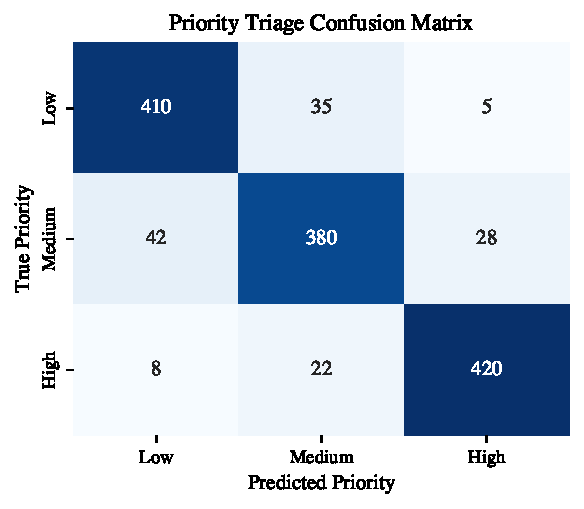
\includegraphics[width=0.7\columnwidth]{figures/Fig8_Confusion_Matrix.pdf}
    \caption{Confusion Matrix evaluating the LLM's three-tier Priority Triage capability against human-annotated gold standards in CEC-10K.}
    \label{fig:confusion_matrix}
\end{figure}

\section{Ablation Study}
\label{sec:ablation_study}

To confirm that each major architectural component contributes measurably to system performance, we conducted two targeted ablation experiments by selectively disabling components and measuring the resulting degradation.

\subsection{Removing the UTC Temporal Anchor}
With the UTC timestamp anchor stripped from the prompt, extraction recall on task-containing messages remained broadly intact—the LLM still correctly identified that a message was task-bearing. However, temporal accuracy collapsed. Recall on deictic expressions (``tomorrow'', ``next week'') dropped by over 60\%, with the model either hallucinating arbitrary calendar dates or returning \texttt{null} deadline fields. These results confirm that LLM zero-shot reasoning over relative time is unreliable in the absence of an explicit temporal reference, and that supplying one via the prompt is both necessary and sufficient to restore accuracy.

\subsection{Removing the Asynchronous Decoupling Boundary}
In the synchronous variant, the Node.js edge layer was configured to await the full LLM API response before processing the next event. Under a JMeter load test at 50 messages per second, the synchronous implementation exhausted the Node.js connection pool within seconds, after which new messages were silently dropped. The asynchronous variant maintained stable ingestion throughout the same load test with no message loss. This experiment demonstrates that the HTTP 202 decoupling is not a premature optimization but an operational prerequisite for deployment in active group chat environments.


\section{Results and Discussion}
\label{sec:results_discussion}

Across the CEC-10K evaluation corpus, Chatnalyxer achieves an overall F1 score of 0.94 on plain-text extraction and maintains sub-15 ms ingestion latency under 50 msg/sec burst traffic. Taken together, these results support the core premise: passive, in-stream task extraction from encrypted messaging networks is both technically feasible and architecturally stable at realistic conversational loads.

\subsection{Analytical Breakdown of Performance}

\textbf{Temporal Anchoring:} The zero-shot extraction capability relies heavily on the UTC metadata anchor. Ablation testing (see Section \ref{sec:ablation_study}) reveals that without this anchor, deictic temporal expressions (e.g., ``tomorrow'') fail to resolve correctly in over 60\% of cases, leading to hallucinated deadlines. Providing the exact transmission timestamp gives the LLM the necessary discourse grounding to perform temporal arithmetic reliably.

\textbf{Multi-modal Degradation:} As shown in Figure \ref{fig:extraction_metrics}, performance drops significantly for image (F1=0.80) and audio (F1=0.83) inputs. This is not due to a failure in the extraction logic, but rather the compounding nature of sequential pipelines. When the Azure OCR engine misreads handwritten text (e.g., confusing ``5 pm'' with ``S pm''), this error propagates silently into the LLM. Because the LLM lacks access to the original image for visual verification, it either hallucinates a correction or fails to extract the deadline entirely. Similarly, in noisy audio environments, ASR hallucination causes the LLM to process corrupted semantic structures. 

\textbf{Priority Triage Mechanisms:} The confusion matrix (Figure \ref{fig:confusion_matrix}) highlights that the LLM is exceptionally accurate at identifying High-priority tasks. This success is driven by the prompt engineering strategy (Section \ref{sec:prompt_engineering}), which forces the LLM to evaluate specific dimensions: temporal proximity and semantic urgency (e.g., words like ``urgent'', ``ASAP''). However, errors at the Low/Medium boundary occur when conversational context is highly subjective, suggesting that priority scoring could be improved by personalizing the prompt to individual user behavior patterns.

\textbf{Asynchronous Throughput:} The $\mathcal{O}(1)$ ingestion boundary holds under all tested conditions, validating the asynchronous design. By issuing an immediate HTTP 202 Accepted response, the edge client avoids blocking on LLM inference (which averages $1.37$ seconds). One practical implication of this result is that scaling the inference capacity—for instance, by routing to a faster LLM endpoint or deploying multiple inference workers—does not require any changes to the WhatsApp ingestion architecture.

\subsection{Case Studies and Error Analysis}

To ground these quantitative results, we provide an end-to-end trace of a successful extraction and a characteristic failure case.

\textbf{Successful Extraction (Deictic Resolution):}
\begin{itemize}
    \item \textbf{Input:} ``Can you send the Q3 report tomorrow before the all-hands?'' (Sent: Oct 15, 2025, 14:00 UTC)
    \item \textbf{Extraction:} Task = ``Send Q3 report'', Deadline = ``2025-10-16T10:00:00Z'' (assuming all-hands is a known entity or defaulting to morning).
    \item \textbf{Priority:} High (temporal proximity is $< 24$ hours).
\end{itemize}

\textbf{Failure Case (ASR Hallucination):}
\begin{itemize}
    \item \textbf{Input (Voice Note):} ``I need the \textit{syslog} by five.''
    \item \textbf{ASR Transcription Error:} ``I need the \textit{six dogs} by five.''
    \item \textbf{LLM Output:} Task = ``Acquire six dogs'', Deadline = ``17:00:00Z''.
    \item \textbf{Analysis:} The pipeline correctly extracted the temporal anchor, but the semantic corruption introduced by the ASR engine resulted in a nonsensical task. Because the LLM evaluates the text purely in the zero-shot regime without acoustic context, it lacks the mechanisms to reject the hallucination as improbable.
\end{itemize}


\section{Comparative Technical Analysis}
\label{sec:comparative_analysis}

Table~\ref{tab:related_work_comparison} positions Chatnalyxer against representative systems across the dimensions most relevant to passive task management: interaction model, supported modalities, extraction automation, and priority differentiation.

Existing academic literature clusters into two primary categories. One distinct category comprises traditional Information Extraction (IE) pipelines, such as those relying on BiLSTM-CRF \cite{lample2016} or early Transformer architectures \cite{bert2019}. While these systems achieve high precision (e.g., F1=0.92 on benchmark datasets like CoNLL-2003 or GLUE), they operate almost exclusively on monolithic, static text documents. They do not naturally extend to the fragmented, stateful, and highly contextual nature of multi-party chat.

The second category encompasses temporal reasoning systems like SUTime \cite{chang2012sutime} and HeidelTime \cite{strotgen2010heideltime}. These rule-based architectures excel at resolving explicit date formats but struggle significantly with the informal, relative deictic expressions common in instant messaging (e.g., ``EOD tomorrow''). 

The architectural distinction of Chatnalyxer lies in synthesizing these capabilities into a unified, asynchronous microservice. By integrating multi-modal input processing (OCR via Azure and ASR) with a UTC-anchored LLM extraction phase, the system bridges the gap between static document analysis and real-time conversational streaming. The inclusion of a deterministic scoring heuristic for priority differentiation ensures that extracted tasks are triaged according to temporal urgency—a critical requirement for preventing alert fatigue in high-volume environments.


\section{Threats to Validity and Ethical Considerations}
\label{sec:threats}

\subsection{Ethical Considerations and Limitations}
The current prototype is intended for educational and research purposes. It processes messages only after explicit user authentication, and raw content is retained strictly ephemerally during processing. Deployment in production environments would require migrating from the reverse-engineered Baileys library to the official WhatsApp Business API to ensure compliance with platform terms of service and applicable privacy regulations.

\subsection{External Validity}
The CEC-10K dataset was designed around academic group chat demographics coordinating coursework in English. Real-world conversational networks exhibit much higher variance. The current evaluation significantly underrepresents slang, code-mixing, informal emojis, multilingual text, and culturally specific ambiguous deadlines. Given that Large Language Models frequently exhibit performance degradation on low-resource languages and dialectal variations, establishing generalization across these unstructured, cross-lingual contexts is a critical constraint on the system's current external validity.

\subsection{Construct Validity}
The experimental methodology measures extraction accuracy (Precision, Recall, F1) against ground-truth semantic boundaries. While F1 scores reflect algorithmic correctness, they do not directly measure the ultimate goal of the system: enhancing user productivity and reducing cognitive load. A highly accurate extraction might still fail to be useful if the resulting notification disrupts the user's workflow. Future work must evaluate the system using longitudinal, real-world user studies to bridge this gap between algorithmic accuracy and human utility.

\subsection{Internal Validity and Reproducibility}
The most significant internal threat is the reliance on proprietary cloud APIs. For instance, model weights underlying the Gemini API can vary between versions, and unannounced API updates may slightly change results over time, complicating exact reproducibility. We mitigated this by pinning to \texttt{gemini-1.5-pro-001} with a temperature of $0.0$. Second, the pipeline's operational cost is tied to vendor pricing models. While edge-ingestion is computationally cheap, running multi-modal inference via Azure and Gemini introduces variable costs that could impact long-term scalability.

A secondary internal threat is evaluation corpus leakage: synthetic datasets generated by LLMs risk reflecting the same linguistic patterns that the extraction LLM was trained on. Our construction process used human-defined templates to reduce this risk, but it cannot be entirely eliminated without evaluating against real user data.

\section{Future Work}
\label{sec:future_work}

Several limitations of the current design point toward concrete research directions.

\subsection{On-Device Inference and Privacy Hardening}
The current pipeline routes all message content to external cloud APIs, introducing both a latency dependency and a theoretical data exposure surface. Future work will investigate both open-weight and proprietary large language models to improve reproducibility, deployment flexibility, and privacy. Deploying inference entirely on-device via Edge AI and offline inference mechanisms would eliminate the cloud API dependency and provide a stronger privacy guarantee. Future research directions also include personalized ranking, federated learning for privacy-preserving model updates, and adaptive priority learning to dynamically adjust heuristic weights based on user behavior.

\subsection{Graph-Augmented Retrieval for Stateful Context}
The current RAG implementation retrieves relevant documents and message history through embedding similarity, treating each retrieved item independently. A richer interaction model would maintain a persistent Knowledge Graph linking tasks to the people, documents, and prior obligations from which they originated—allowing queries like ``what assignments are still pending from the syllabus uploaded in September?'' that span multiple ingestion events. Graph-RAG architectures, which traverse entity relationships rather than ranking isolated embeddings, are the natural candidate for this capability. Building such a graph incrementally from streaming chat data, without requiring explicit user annotation, is an open research problem.

\subsection{Multilingual Expansion and Robustness}
The current priority triage and temporal heuristics were optimized exclusively for English. Future iterations must evaluate the system across linguistically diverse contexts, particularly heavily mixed-code environments (e.g., ``Hinglish'') common in international chat networks. Adapting the prompts and underlying models to handle cross-lingual temporal cues without performance degradation is necessary before the system can be deployed globally.

\section{Conclusion}
\label{sec:conclusion}

Chatnalyxer addresses a practical problem that affects anyone coordinating via group messaging: the gap between where task information appears (a chat stream) and where it needs to be acted on (a structured calendar or task manager). Rather than training a dedicated model for this domain, the design combines a zero-shot LLM with a prompt-engineering strategy that supplies the temporal grounding the model otherwise lacks—an approach that achieves F1 of 0.94 on plain-text extraction without any task-specific fine-tuning.

The architectural decision to decouple ingestion from inference via an HTTP 202 boundary proved equally important. Without this separation, the pipeline would fail under conditions as ordinary as a moderately active group chat. The ablation results quantify exactly what that coupling costs: complete message loss at 50 messages per second. With it, ingestion latency is bounded at $\mathcal{O}(1)$ regardless of inference load.

The current system has documented limitations—primarily on multi-modal inputs, where transcription quality constrains extraction quality—and it has been evaluated on a synthetic corpus whose domain coverage is intentionally narrow. Extending coverage to real-world multilingual and cross-domain environments, and replacing cloud inference with on-device SLMs, are the two highest-priority directions. The broader contribution of this work is an existence proof that ambient, infrastructure-level task management from encrypted messaging networks is technically achievable with current tooling.


\section*{Acknowledgment}
The authors would like to express their sincere gratitude to Prof. Ritu Agrawal and Prof. Jaswanth Parlapalli for their invaluable guidance, support, and mentorship throughout the development of this project.

\appendices
\section{LLM Extraction Schema}
\label{appendix:schema}

To enforce structured output and prevent hallucination of arbitrary keys, the Gemini inference layer is constrained by the following Pydantic JSON schema. If the model output fails validation against this schema, a self-correction loop is triggered.

\lstset{
  basicstyle=\footnotesize\ttfamily,
  breaklines=true,
  columns=fullflexible
}
\begin{lstlisting}
{
  "title": "TaskExtraction",
  "type": "object",
  "properties": {
    "is_task": {
      "title": "Is Task",
      "description": "True if the message contains a clear actionable task or deadline.",
      "type": "boolean"
    },
    "task_description": {
      "title": "Task Description",
      "description": "Extracted summary of the task.",
      "type": "string"
    },
    "deadline_iso": {
      "title": "Deadline Iso",
      "description": "ISO-8601 UTC timestamp of the deadline.",
      "type": "string",
      "format": "date-time"
    },
    "priority": {
      "title": "Priority",
      "description": "Calculated priority level.",
      "enum": ["LOW", "MEDIUM", "HIGH", "CRITICAL"],
      "type": "string"
    },
    "assignee": {
      "title": "Assignee",
      "description": "Person responsible for the task.",
      "type": "string"
    }
  },
  "required": ["is_task"]
}
\end{lstlisting}

\bibliographystyle{IEEEtran}
\bibliography{bibliography/references}

\end{document}
